\section{Avbrudd}
\label{sec:avbrudd}
Eksterne avbrytelser refererer til situasjoner hvor eksterne hendelser forstyrrer pågående aktiviteter \citep{Harr07}. Da mange arbeidsaktiviteter er kognitive, altså krever tenkning, problemløsing og evnen til å forutse og ta beslutninger, argumenterer \citet{Rogers94} for at det kreves en forståelse for hvordan disse aktivitetene utføres for å kunne designe datasystemer som kan støtte både kognitive aktiviteter og sosial interaksjon.

\tikzstyle{mybox} = [draw=black, fill=white, very thick,
    rectangle, inner sep=10pt, inner ysep=20pt, rounded corners]
\tikzstyle{fancytitle} =[fill=black, text=white]
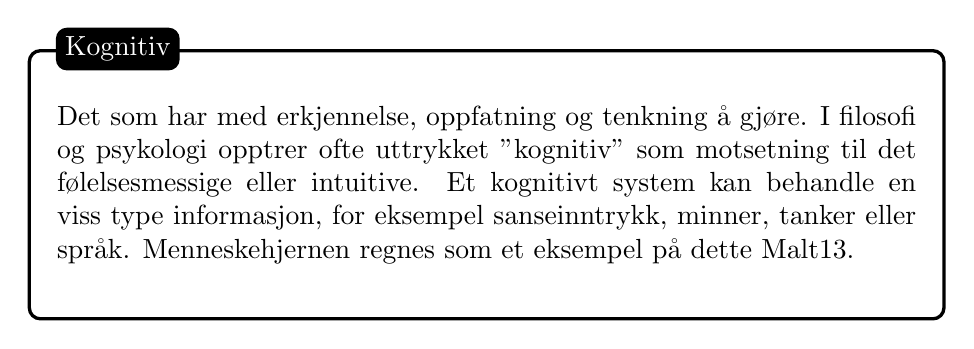
\begin{tikzpicture}
\node [mybox] (box){%
    \begin{minipage}{0.9\textwidth}
     Det som har med erkjennelse, oppfatning og tenkning å gjøre. I filosofi og psykologi opptrer ofte uttrykket $"$kognitiv$"$ som motsetning til det følelsesmessige eller intuitive. Et kognitivt system kan behandle en viss type informasjon, for eksempel sanseinntrykk, minner, tanker eller språk. Menneskehjernen regnes som et eksempel på dette \citep{Malt13}.
    \end{minipage}
};
\node[fancytitle, rounded corners, right=10pt] at (box.north west) {Kognitiv};
\end{tikzpicture}%

\noindent
Det skilles normalt mellom langtids- og korttidsminne. Den passive kunnskapen man besitter ligger i langtidsminnet, for eksempel medisinske fakta eller viktige datoer. Kortidsminnet, eller arbeidsminnet, er den bevisste delen av minnet som aktivt behandler informasjon. Arbeidsminnet har begrenset kapasitet og varighet, og lar seg raskt forstyrre av distraksjoner og avbrytelser \citep{Parker00}. \citet{Coiera98} antyder at synkron kommunikasjon, ansikt-til-ansikt eller per telefon, foretrekkes fordi det gir en umiddelbar bekreftelse på at en beskjed er mottatt. Dersom man ønsker å gi en beskjed eller et ansvar videre, vil usikkerheten om beskjeden er mottatt bli liggende i arbeidsminnet frem til man får en bekreftelse fra mottaker. 

\noindent
“Stacking” defineres som den usynlige beslutningsprosessen sykepleiere utfører om hva, hvordan og når de skal gi pleie til en tildelt gruppe pasienter \citep{Ebright10}. Stadige endringer i omgivelser og informasjonsflyt resulterer i en kontinuerlig omprioritering av hvilke oppgaver som skal utføres når. Dette kombinert med avbrytelser fra omgivelsene, kan resultere i en kognitiv belastning som kan hemme oppmerksomheten \citep{Ebright10}. \citet{Parker00} hevder at en begrensende faktor i enhver kommunikasjonsanalyse er den kognitive kapasiteten individer har til å gjennomføre sitt arbeid, da studier har vist at feil og ineffektivitet er et resultat av at denne kapasiteten overskrides. Kunnskap om menneskets hukommelse hevdes å være nøkkelen til å forstå hvilke krav som bør settes til teknologi brukt i slike omgivelser.

\subsection{Dualiteten ved avbrudd}
\citet{Grundgeiger09} skiller mellom gode og dårlige avbrudd, og hevder disse må sees i sammenheng med hvilke effekter de har. Eksempler på positive effekter er øyeblikkelig kommunikasjon og tilgang til viktig informasjon. Avbryter opplever å få en umiddelbar bekreftelse på at informasjonen er mottatt og kan dermed avlaste arbeidsminnet, mens den som blir avbrutt kan oppleve negative effekter, som overbelastet kognitiv kapasitet, forsinkelse i eget arbeid, stress og frustrasjon. Samtidig kan avbruddet ha en positiv effekt dersom den avbrutte mottar ønsket informasjon.

\noindent
\citet{Harr07} presenterer fire ulike typer avbrytelser: (1) mellommenneskelige relasjoner, (2) lokasjon, (3) frysing og (4) samarbeid.

\noindent
Generelt vil avbryter vurdere situasjonen, og avgjøre om avbruddet bør initieres. Denne prosessen vil delvis være påvirket av relasjonen som allerede eksisterer mellom avbryter og den som avbrytes, illustrert i figur \ref{interpersonal}. Faktorer som kan påvirke adferden til de to partene er maktforhold, arbeidsrolle, hastegrad, normer, regler og vennskap. 
\begin{figure}[H]
\centering
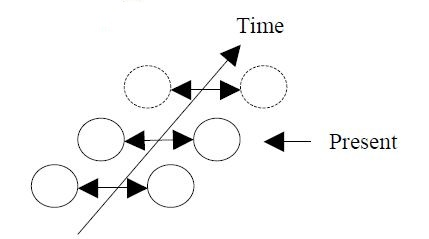
\includegraphics[scale=0.5]{interpersonal.jpg}
\caption{Mellommenneskelige relasjoner}
\label{interpersonal}
\end{figure}

\noindent
Avbrudd kan også ha effekt på andre som befinner seg på samme lokasjon som den som blir avbrutt. Dette illustreres i figur \ref{collateral}, hvor interaksjonen mellom aktør D (avbryter) og aktør B (den som avbrytes) også påvirker aktørene A og C.
\begin{figure}[H]
\centering
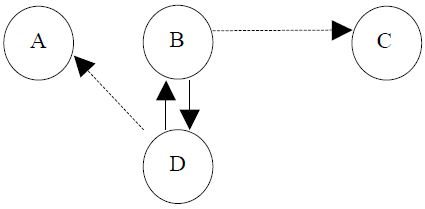
\includegraphics[scale=0.5]{collateral.jpg}
\caption{Lokasjonsbasert forstyrrelse}
\label{collateral}
\end{figure}

\noindent
En annen situasjon som kan oppstå er det som kalles frysing. Dersom aktører B og C utfører en oppgave ved synkron kommunikasjon, eksempelvis ansikt-til-ansikt eller per telefon, og aktør A avbryter aktør B, vil aktør C måtte vente til aktør B igjen blir tilgjengelig. 
\begin{figure}[H]
\centering
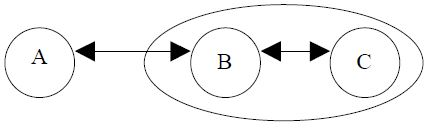
\includegraphics[scale=0.5]{frysing.jpg}
\caption{Frysing}
\label{frysing}
\end{figure}

\noindent
For en gruppe som samarbeider, vil oppgaver utført av et enkelt individ ofte være deler av den overordnede kollektive aktiviteten. Dermed vil forstyrrelsen av et individ sannsynligvis påvirke andre medlemmer i gruppen. Figur \ref{direkte} viser aktør B og aktør C som samarbeider om en oppgave GT, hvor GT er en del av den overordnede aktiviteten CA. Dersom aktør A avbryter aktør B, vil aktør C kanskje måtte dekke for aktør B, frem til B igjen blir tilgjengelig.
\begin{figure}[H]
\centering
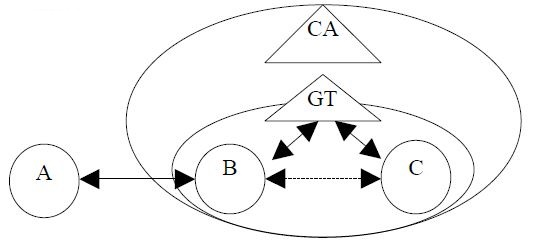
\includegraphics[scale=0.5]{coverme.jpg}
\caption{Samarbeid og avbrudd - direkte forstyrrelse}
\label{direkte}
\end{figure}

\noindent
Aktørene B og C må ikke nødvendigvis kommunisere direkte, men aktør C kan være avhengig av tiden, innholdet og kvaliteten aktør Bs oppgave resulterer i. Dermed kan en forstyrrelse av aktør B også indirekte forstyrre aktør C.
\begin{figure}[H]
\centering
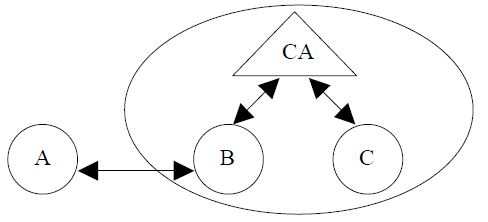
\includegraphics[scale=0.5]{dropball.jpg}
\caption{Samarbeid og avbrudd - indirekte forstyrrelse}
\label{indirekte}
\end{figure}

\subsection{Avbruddshåndtering}
Gitt dualiteten ved avbrudd kan avbruddshåndtering sies å ha to mål: (1) redusere de negative effektene, og (2) utnytte de positive effektene ved avbrudd. \citet{Grandhi10} gir fire teknikker for avbruddshåndtering:
\begin{enumerate}        
\item Forebygging - bruk av funksjoner som forebygger eller blokkerer innkommende avbrytelser. Dette kan gjøres enkelt ved å for eksempel skru av mobilen for en periode. En annen strategi er å kontrollere timingen til avbruddet eller å kun tillate avbrytelser som er relevant for den oppgaven man utfører.

\item Fraråding - bruk av funksjoner som fraråder avbrytelser. Dette skjer ofte ved at man gir informasjon til avbryter om tilgjengeligheten til den man ønsker å avbryte. 

\item Modifiserte varslinger - bruk av funksjoner som modifiserer hvordan individer varsles om innkommende anrop. Ved bruk av ulike modaliteter som lyd, vibrasjon og lys, kan man minimere interferensen mellom perseptuelle og kognitive prosesser involvert i avbruddshåndtering og oppgaveytelse \citep{Harr07}.

\item Forhåndsvisning - bruk av funksjoner som gir informasjon om selve avbrytelsen som den avbrutte selv kan reflektere over.   
\end{enumerate}

